%==============================================================================
%  LEGAL RAG SYSTEM — TECHNICAL SYSTEM REPORT
%  Author : Abdul Ghafoor  |  skillSYNC AI/ML Internship — Pair B
%  Scope  : backendd/ (FastAPI orchestration core) + frontendd/ (React client)
%  Engine : pdfLaTeX  (compiles as-is on Overleaf, no external assets required)
%==============================================================================
\documentclass[11pt,a4paper]{article}

% ── Page geometry ────────────────────────────────────────────────────────────
\usepackage[top=2.1cm,bottom=1.85cm,left=2.05cm,right=2.05cm,headsep=11pt]{geometry}
\usepackage[T1]{fontenc}
\usepackage[utf8]{inputenc}
\usepackage{lmodern}
\usepackage{microtype}
\usepackage{parskip}
\usepackage{ragged2e}

% ── Palette ──────────────────────────────────────────────────────────────────
\usepackage{xcolor}
\definecolor{ink}        {HTML}{0B1220}
\definecolor{navy}       {HTML}{143C6E}
\definecolor{azure}      {HTML}{0070A4}
\definecolor{gold}       {HTML}{B98A2E}
\definecolor{riskred}    {HTML}{AA2323}
\definecolor{amber}      {HTML}{B85C00}
\definecolor{forest}     {HTML}{1E6E37}
\definecolor{slate}      {HTML}{4B5563}
\definecolor{mist}       {HTML}{F4F6FA}
\definecolor{hairline}   {HTML}{D8DEE9}
\definecolor{codebg}     {HTML}{FBFCFE}

% ── Typography of headings ───────────────────────────────────────────────────
\usepackage{titlesec}
\titleformat{\section}[hang]
  {\Large\bfseries\color{navy}}
  {\color{gold}\thesection\hspace{0.55em}}{0pt}{}
  [\vspace{-6pt}{\color{navy}\rule{\linewidth}{1.1pt}}\vspace{-2pt}]
\titleformat{\subsection}[hang]
  {\normalsize\bfseries\color{azure}}{\thesubsection}{0.6em}{}
\titleformat{\subsubsection}[runin]
  {\small\bfseries\color{slate}}{}{0em}{}[.\hspace{0.4em}]
\titlespacing*{\section}{0pt}{9pt}{4pt}
\titlespacing*{\subsection}{0pt}{7pt}{1pt}
\usepackage{multicol}

% ── Headers / footers ────────────────────────────────────────────────────────
\usepackage{fancyhdr}
\setlength{\headheight}{15pt}
\pagestyle{fancy}\fancyhf{}
\fancyhead[L]{\footnotesize\color{slate}\textsc{Legal RAG System}\;\textcolor{hairline}{|}\;Technical System Report}
\fancyhead[R]{\footnotesize\color{slate}Abdul Ghafoor \textcolor{hairline}{|} Pair B}
\fancyfoot[C]{\footnotesize\color{slate}\thepage}
\renewcommand{\headrulewidth}{0.6pt}
\renewcommand{\headrule}{\hbox to\headwidth{\color{hairline}\leaders\hrule height \headrulewidth\hfill}}

% ── Tables ───────────────────────────────────────────────────────────────────
\usepackage{booktabs}
\usepackage{tabularx}
\usepackage{array}
\usepackage{colortbl}
\usepackage{multirow}
\newcolumntype{L}[1]{>{\RaggedRight\arraybackslash}p{#1}}
\newcolumntype{C}[1]{>{\Centering\arraybackslash}p{#1}}
\renewcommand{\arraystretch}{1.02}

% ── Boxes ────────────────────────────────────────────────────────────────────
\usepackage[most]{tcolorbox}
\tcbuselibrary{skins,breakable}

\newtcolorbox{keybox}[1]{enhanced,breakable,colback=azure!5,colframe=azure,
  boxrule=0.8pt,arc=3pt,left=8pt,right=8pt,top=6pt,bottom=6pt,
  fonttitle=\bfseries\footnotesize\color{white},title={#1},
  attach boxed title to top left={xshift=8pt,yshift=-8pt},
  boxed title style={colback=azure,arc=2pt,boxrule=0pt}}

\newtcolorbox{riskbox}[1]{enhanced,breakable,colback=riskred!5,colframe=riskred,
  boxrule=0.8pt,arc=3pt,left=8pt,right=8pt,top=6pt,bottom=6pt,
  fonttitle=\bfseries\footnotesize\color{white},title={#1},
  attach boxed title to top left={xshift=8pt,yshift=-8pt},
  boxed title style={colback=riskred,arc=2pt,boxrule=0pt}}

\newtcolorbox{winbox}[1]{enhanced,breakable,colback=forest!5,colframe=forest,
  boxrule=0.8pt,arc=3pt,left=8pt,right=8pt,top=6pt,bottom=6pt,
  fonttitle=\bfseries\footnotesize\color{white},title={#1},
  attach boxed title to top left={xshift=8pt,yshift=-8pt},
  boxed title style={colback=forest,arc=2pt,boxrule=0pt}}

\newtcolorbox{quietbox}{enhanced,breakable,colback=mist,colframe=hairline,
  boxrule=0.7pt,arc=3pt,left=8pt,right=8pt,top=6pt,bottom=6pt}

% Metric tile used on the dashboard page
\newcommand{\metric}[3]{%
  \begin{minipage}[t]{0.235\linewidth}%
  \begin{tcolorbox}[width=\linewidth,height=1.85cm,valign=center,halign=center,
    colback=white,colframe=#3,boxrule=1pt,arc=3pt,left=1pt,right=1pt,top=1pt,bottom=1pt]
    {\fontsize{15}{15}\selectfont\bfseries\color{#3}#1}\\[2pt]
    {\scriptsize\color{slate}#2}
  \end{tcolorbox}%
  \end{minipage}}

% ── Graphics & diagrams ──────────────────────────────────────────────────────
\usepackage{tikz}
\usetikzlibrary{arrows.meta,positioning,shapes.geometric,calc,fit,backgrounds,shadows.blur}
\usepackage{float}

% ── Lists ────────────────────────────────────────────────────────────────────
\usepackage{enumitem}
\setlist[itemize]{leftmargin=1.25em,itemsep=1.5pt,topsep=3pt}
\setlist[enumerate]{leftmargin=1.45em,itemsep=1.5pt,topsep=3pt}

% ── Code ─────────────────────────────────────────────────────────────────────
\usepackage{listings}
\lstdefinelanguage{JavaScript}{
  keywords={const,let,var,async,await,function,return,if,else,useRef,useEffect,setInterval,clearInterval,new,export,default},
  ndkeywords={true,false,null,undefined},
  sensitive=true,
  comment=[l]{//},morecomment=[s]{/*}{*/},
  morestring=[b]',morestring=[b]",morestring=[b]`
}
\lstdefinestyle{src}{
  backgroundcolor=\color{codebg},basicstyle=\scriptsize\ttfamily,
  breaklines=true,frame=leftline,framerule=1.6pt,rulecolor=\color{azure!45},
  keywordstyle=\color{navy}\bfseries,commentstyle=\color{forest}\itshape,
  stringstyle=\color{riskred},showstringspaces=false,tabsize=2,
  xleftmargin=9pt,aboveskip=6pt,belowskip=4pt,columns=fullflexible}
\lstset{style=src}

% ── Captions & links ─────────────────────────────────────────────────────────
\usepackage[font=small,labelfont={bf,color=navy},skip=4pt]{caption}
\usepackage{hyperref}
\hypersetup{colorlinks=true,linkcolor=azure,urlcolor=azure,citecolor=azure,
  pdftitle={Legal RAG System — Technical System Report},
  pdfauthor={Abdul Ghafoor}}

% ── Shorthands ───────────────────────────────────────────────────────────────
\newcommand{\code}[1]{\texttt{\small #1}}
\newcommand{\pkr}{PKR\,}
\newcommand{\HI}{\textcolor{riskred}{\textbf{HIGH}}}
\newcommand{\ME}{\textcolor{amber}{\textbf{MEDIUM}}}
\newcommand{\LO}{\textcolor{forest}{\textbf{LOW}}}

%==============================================================================
\begin{document}

% ─────────────────────────── TITLE PAGE ─────────────────────────────────────
\begin{titlepage}
\thispagestyle{empty}
\begin{tikzpicture}[remember picture,overlay]
  \fill[ink] (current page.north west) rectangle ($(current page.north east)+(0,-9.6cm)$);
  \fill[gold] ($(current page.north west)+(0,-9.6cm)$) rectangle ($(current page.north east)+(0,-9.75cm)$);
  \begin{scope}
    \clip ($(current page.north west)$) rectangle ($(current page.north east)+(0,-9.6cm)$);
    \foreach \i in {0,...,14}{
      \draw[azure!22,line width=0.5pt] ($(current page.north west)+(\i*1.6cm,-1.2cm)$)
        -- ++(0.9cm,-1.1cm) -- ++(0,-2.3cm) -- ++(1.0cm,-1.2cm);
      \fill[gold!45] ($(current page.north west)+(\i*1.6cm+0.9cm,-2.3cm)$) circle (1.5pt);}
  \end{scope}
  \node[anchor=north west,text width=15cm] at ($(current page.north west)+(2.3cm,-2.1cm)$)
    {\color{gold}\footnotesize\bfseries\sffamily
     RETRIEVAL-AUGMENTED GENERATION \; \textbullet \; PAKISTANI LEGAL DOMAIN};
  \node[anchor=north west,text width=16cm] at ($(current page.north west)+(2.25cm,-3.0cm)$)
    {\color{white}\fontsize{31}{36}\selectfont\bfseries Legal RAG System};
  \node[anchor=north west,text width=15.5cm] at ($(current page.north west)+(2.3cm,-5.4cm)$)
    {\color{white!80}\fontsize{14}{19}\selectfont
     An AI-Assisted Due Diligence Engine for Property, Lending and\\ Corporate Acquisition Transactions};
  \node[anchor=north west,text width=15cm] at ($(current page.north west)+(2.35cm,-7.6cm)$)
    {\color{azure!70}\small\itshape Architecture, hardening and verification of the
     \code{backendd} orchestration core and \code{frontendd} client};
\end{tikzpicture}

\vspace*{8.6cm}

\begin{center}\small
\begin{tabularx}{0.94\linewidth}{@{}>{\bfseries\color{navy}}l X@{}}
\toprule
Author            & Abdul Ghafoor \\
Programme         & skillSYNC AI/ML Engineering Internship --- Pair B \\
Deliverable       & Technical System Report (individual contribution) \\
Repository scope  & \code{backendd/} (Python 3.11+ / FastAPI) and \code{frontendd/} (React 19 / Vite 8) \\
Out of scope      & \code{backend/} --- a parallel implementation authored by the paired teammate \\
Build history     & Prototype 29 June --- 05 July 2026; hardening pass August 2026 \\
Date of report    & \today \\
\bottomrule
\end{tabularx}
\end{center}

\vspace{0.75cm}

\begin{center}
\metric{11{,}169}{lines first-party}{navy}\hfill
\metric{303}{tests passing}{forest}\hfill
\metric{2{,}510}{statute vectors}{azure}\hfill
\metric{9}{red-flag rules}{riskred}
\end{center}

\vfill
\begin{center}
{\color{hairline}\rule{0.5\linewidth}{0.6pt}}\\[6pt]
{\footnotesize\color{slate}
Every quantitative figure in this report is read from the committed source tree, the
persisted vector store or an actual test run --- never projected.\\
Section~\ref{sec:defects} states what was defective; Section~\ref{sec:critical} states
what still is.}
\end{center}
\vspace{0.4cm}
\end{titlepage}

% ─────────────────────────── ABSTRACT + TOC ─────────────────────────────────
\section*{\color{navy}Abstract}
\vspace{-6pt}{\color{gold}\rule{\linewidth}{1.1pt}}\vspace{2pt}

\noindent
First-pass legal due diligence is structurally inefficient: a senior associate reads a
bundle of thirty to fifty scanned pages, answers the same fifteen questions that were
answered on the previous mandate, and writes those answers into a memorandum whose
skeleton has not changed in a decade. The work is expensive, slow, linguistically awkward
in a jurisdiction where title records are frequently handwritten in Urdu, and ---
because it is performed under deadline --- measurably error-prone.

This report documents the \textbf{Legal RAG System}: a retrieval-augmented generation
pipeline that ingests a lawyer's PDF bundle, indexes it alongside a persistent corpus of
Pakistani primary legislation, interrogates both corpora with a jurisdiction-aware
diligence checklist, and emits a branded, citation-bearing memorandum in Word and PDF.
The architectural commitment that defines it is \emph{dual-corpus fusion}: every question
retrieves from the client's own documents \emph{and} from a statutory index built on the
Constitution of Pakistan 1973, the Transfer of Property Act 1882, the Registration Act
1908 and the Stamp Act 1899, so a finding is never a bare assertion --- it carries a
document citation, a statutory citation and a constitutional article together.

The system described here is the product of a five-day prototype followed by a
systematic hardening pass, and this report is organised around that distinction.
Section~\ref{sec:defects} is a defect register: nineteen concrete faults found in the
prototype --- among them a path-traversal vulnerability in the upload handler, an
unauthenticated route serving privileged memoranda, negation-blind rules that raised red
flags asserting the opposite of what a document said, and monetary extraction that read
national identity numbers as rupee amounts and tripped a statutory money-laundering
threshold --- each with the change that closed it. The remaining sections document the
resulting system: 11{,}169 lines of first-party code, ten HTTP routes, durable SQLite
session state, a shared token-bucket limiter, a WCAG-conformant responsive interface, and
a 303-case test suite that runs green without a model, a GPU or a network.
Section~\ref{sec:critical} states without hedging what the system still does not do.

\vspace{2pt}
\begin{quietbox}
\footnotesize
\textbf{Keywords:} retrieval-augmented generation; legal informatics; vector search;
cross-encoder reranking; multilingual OCR; Pakistani property law; document automation;
FastAPI; LlamaIndex; ChromaDB; software hardening.
\end{quietbox}

\vspace{6pt}
{\color{navy}\large\bfseries Contents}\vspace{-6pt}\\
{\color{gold}\rule{\linewidth}{1.1pt}}
\vspace{-20pt}
{\footnotesize\setlength{\parskip}{0pt}\renewcommand{\contentsname}{}
 \setcounter{tocdepth}{1}
 \begin{multicols}{2}\tableofcontents\end{multicols}}

\newpage

% ═══════════════════════════════════════════════════════════════════════════
\section{Introduction and Problem Formulation}
% ═══════════════════════════════════════════════════════════════════════════

\subsection{The task being automated}

A property due diligence review in Pakistan is neither a search problem nor a
summarisation problem. It is a \emph{structured interrogation} problem: the lawyer does not
ask ``what does this document say'' but works through a fixed, professionally mandated
sequence of questions --- is the title registered, is it encumbered, is the NOC present, is
the mutation recorded --- answering each with an evidentiary trail back to a page of a
document and forward to a section of a statute.

That framing dictates the architecture. A conversational assistant is the wrong shape: the
output is a memorandum with a fixed section order that a partner will sign. The right shape
is a pipeline whose final artefact is a document, whose intermediate representation is a
list of schema-conformant findings, and whose retrieval layer reaches two knowledge bases
at once.

\subsection{Why the jurisdiction is the interesting constraint}

Three jurisdictional facts drive most of the non-obvious engineering.

\begin{enumerate}
\item \textbf{Bilingual, frequently non-digital records.} Revenue documents ---
\emph{Fard-e-Malkiat}, \emph{Intiqal}, \emph{Jamabandi} --- are routinely scans of Urdu
manuscript. A pipeline assuming extractable Latin text fails on the first real bundle.

\item \textbf{Authority fragmentation.} The controlling authority, required NOCs and
governing bye-laws all change with the city --- CDA in Islamabad, RDA in Rawalpindi, LDA in
Lahore, SBCA in Karachi --- so a single national checklist is legally wrong.

\item \textbf{Statutory thresholds with numeric triggers.} Withholding tax under
sections 236C and 236K of the Income Tax Ordinance 2001 attaches above \pkr 5{,}000{,}000;
enhanced due diligence under the Anti-Money Laundering Act 2010 attaches above
\pkr 10{,}000{,}000. These are arithmetic conditions on a value that must first be
extracted from prose expressing it as ``50 lakh'' or ``1 crore''.
\end{enumerate}

\begin{keybox}{Design thesis}
\small
Retrieval-augmented generation is used here not to make the system \emph{conversational}
but to make it \emph{accountable}. Every field in the output schema exists so that a
reviewing advocate can falsify the machine's claim in under a minute. The system is
optimised for verifiability, not fluency --- and, as Section~\ref{sec:defects} shows,
that principle is also what made its early defects findable.
\end{keybox}

% ═══════════════════════════════════════════════════════════════════════════
\section{Defect Register}
\label{sec:defects}
% ═══════════════════════════════════════════════════════════════════════════

The prototype reached a working vertical slice in five days. A subsequent audit of that
slice found nineteen defects, several of them serious. This section records them and the
change that closed each, because a report that describes only the finished artefact hides
the part of the engineering that actually mattered.

\begin{table}[H]
\centering\scriptsize
\begin{tabularx}{\linewidth}{@{}>{\ttfamily}c L{5.5cm} X@{}}
\toprule
\rowcolor{mist}\normalfont\textbf{ID} & \textbf{Defect} & \textbf{Resolution} \\
\multicolumn{3}{@{}l}{\color{riskred}\bfseries\normalfont Security} \\
\midrule
D01 & Path traversal: upload filenames used verbatim, so \code{../../core/main.py} overwrote application source & Sanitiser strips directory components, control characters and reserved names; destination asserted under the upload root \\
D02 & Privileged memoranda served unauthenticated behind an 8-character (32-bit) session id & 256-bit \code{token\_urlsafe} identifiers; optional constant-time API-key check on every session route \\
D03 & Extension-only file validation accepted a renamed \code{.docx} & Magic-byte validation on the first streamed chunk, server- and client-side \\
D04 & \code{await file.read()} loaded whole files into memory before the size check & 1\,MiB streaming with per-file and bundle limits enforced mid-stream \\
\midrule
\multicolumn{3}{@{}l}{\color{riskred}\bfseries\normalfont Correctness} \\
\midrule
D05 & Negation-blind rules: \emph{``no ongoing litigation''} raised the litigation flag & Word-boundary regex with a negation window and clause-boundary scope reset; rules also evaluate source text \\
D06 & A 13-digit CNIC parsed as rupees and tripped the \pkr 10\,M AML threshold & Currency cue required; CNIC/IBAN/card patterns masked; implausible values rejected \\
D07 & \code{LLMSingleSelector} routed each question to exactly one corpus & Both indexes queried concurrently and fused; the routing call is eliminated \\
D08 & \code{city\_profiles.json} and \code{housing\_societies.json} written but never read & Questions templated against the selected authority and the detected society's document list \\
D09 & \code{Settings.llm} mutated globally on every call, racing under concurrency & The model is passed explicitly at every call site \\
D10 & A fresh embedding model built on every index build and every query & Process-wide singleton behind a lock \\
D11 & Chunking left to library defaults despite documentation promising 512/50 & Explicit \code{SentenceSplitter} from settings, pinned by a test \\
D12 & The statutory corpus could never be rebuilt; adding a PDF had no effect & Corpus fingerprinted by name, size and mtime; a change triggers exactly one rebuild \\
\midrule
\multicolumn{3}{@{}l}{\color{riskred}\bfseries\normalfont Reliability} \\
\midrule
D13 & Session state in module dictionaries died with the process and blocked multi-worker runs & WAL-mode SQLite store; indexes rebuilt on demand from the persisted collection \\
D14 & \code{time.sleep(4)} per question: not adaptive, ignored 429s, unshared across sessions & Shared token bucket over both ceilings, plus jittered backoff honouring \code{Retry-After} \\
D15 & Cleanup ran only on upload, so idle deployments kept expired privileged documents & Periodic worker on the application lifespan, plus an explicit delete route \\
D16 & \code{create\_task} results discarded, so pipeline crashes vanished and clients polled forever & Tasks tracked, drained on shutdown, failures written to the session \\
\midrule
\multicolumn{3}{@{}l}{\color{riskred}\bfseries\normalfont Interface} \\
\midrule
D17 & \code{setInterval} polling overlapped requests; network blips were silently ignored & Self-scheduling poll with failure counting, backoff and abort-on-unmount \\
D18 & No focus styles, no keyboard access, tabs unlabelled to assistive technology & WCAG 2.2 AA focus rings, WAI-ARIA tabs with arrow keys, live regions for progress and errors \\
D19 & Fixed desktop layout overflowed below roughly 900\,px & Mobile-first rebuild with breakpoints at 640, 720 and 900\,px, verified at three viewports \\
\bottomrule
\end{tabularx}
\caption{Defect register. Nineteen faults found by audit of the prototype, with the change that closed each. The security and correctness classes carry regression tests named after the failure they pin.}
\label{tab:defects}
\end{table}

% ═══════════════════════════════════════════════════════════════════════════
\section{System Architecture}
% ═══════════════════════════════════════════════════════════════════════════

\subsection{Topology}

The system is a four-tier pipeline with a single asynchronous orchestrator. A browser
client posts a multipart bundle; FastAPI validates and persists it, mints a session and
returns immediately while the expensive work proceeds on a background task; the client
then polls a status endpoint until completion. This \emph{fire-and-poll} shape is
deliberate --- the pipeline runs for minutes, far beyond any reasonable HTTP timeout.

\begin{figure}[H]
\centering
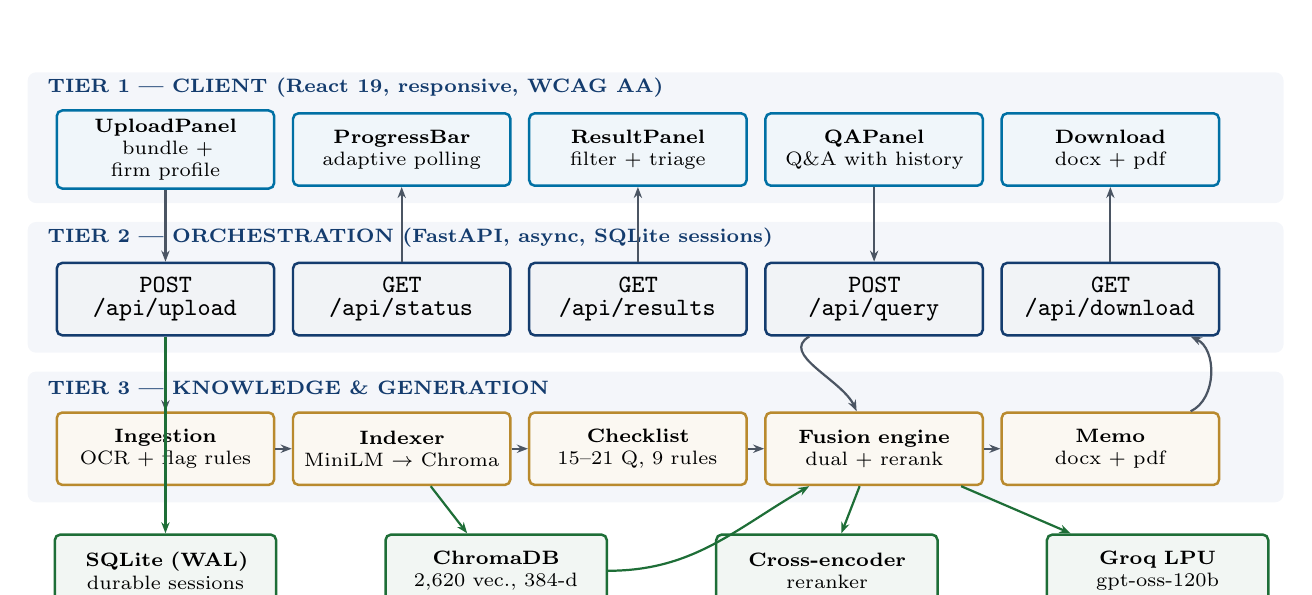
\begin{tikzpicture}[
  font=\scriptsize,
  box/.style={draw=#1,fill=#1!6,line width=0.9pt,rounded corners=2pt,
              text width=2.55cm,align=center,minimum height=0.92cm,inner sep=3pt},
  ar/.style={-{Stealth[length=4pt]},line width=0.8pt,draw=slate},
  lab/.style={font=\scriptsize\bfseries\color{navy}}
]
\fill[mist,rounded corners=3pt] (-0.35,-0.68) rectangle (15.6,0.98);
\fill[mist,rounded corners=3pt] (-0.35,-2.58) rectangle (15.6,-0.92);
\fill[mist,rounded corners=3pt] (-0.35,-4.48) rectangle (15.6,-2.82);

\node[lab,anchor=west] at (-0.22,0.78) {TIER 1 \textemdash{} CLIENT (React 19, responsive, WCAG AA)};
\node[lab,anchor=west] at (-0.22,-1.12) {TIER 2 \textemdash{} ORCHESTRATION (FastAPI, async, SQLite sessions)};
\node[lab,anchor=west] at (-0.22,-3.02) {TIER 3 \textemdash{} KNOWLEDGE \& GENERATION};

\node[box=azure]  (up) at (1.4,0.0)  {\textbf{UploadPanel}\\bundle + firm profile};
\node[box=azure]  (pb) at (4.4,0.0)  {\textbf{ProgressBar}\\adaptive polling};
\node[box=azure]  (rp) at (7.4,0.0)  {\textbf{ResultPanel}\\filter + triage};
\node[box=azure]  (qa) at (10.4,0.0) {\textbf{QAPanel}\\Q\&A with history};
\node[box=azure]  (dl) at (13.4,0.0) {\textbf{Download}\\docx + pdf};

\node[box=navy]   (ep) at (1.4,-1.9)  {\code{POST}\\\code{/api/upload}};
\node[box=navy]   (st) at (4.4,-1.9)  {\code{GET}\\\code{/api/status}};
\node[box=navy]   (rs) at (7.4,-1.9)  {\code{GET}\\\code{/api/results}};
\node[box=navy]   (qy) at (10.4,-1.9) {\code{POST}\\\code{/api/query}};
\node[box=navy]   (dn) at (13.4,-1.9) {\code{GET}\\\code{/api/download}};

\node[box=gold]   (dp) at (1.4,-3.8)  {\textbf{Ingestion}\\OCR + flag rules};
\node[box=gold]   (ix) at (4.4,-3.8)  {\textbf{Indexer}\\MiniLM $\rightarrow$ Chroma};
\node[box=gold]   (ck) at (7.4,-3.8)  {\textbf{Checklist}\\15--21 Q, 9 rules};
\node[box=gold]   (qe) at (10.4,-3.8) {\textbf{Fusion engine}\\dual + rerank};
\node[box=gold]   (mg) at (13.4,-3.8) {\textbf{Memo}\\docx + pdf};

\draw[ar] (up) -- (ep);  \draw[ar] (st) -- (pb);
\draw[ar] (rs) -- (rp);  \draw[ar] (qa) -- (qy);  \draw[ar] (dn) -- (dl);
\draw[ar] (ep) -- (dp);  \draw[ar] (dp) -- (ix);  \draw[ar] (ix) -- (ck);
\draw[ar] (ck) -- (qe);  \draw[ar] (qe) -- (mg);
\draw[ar] (mg) to[out=25,in=-25] (dn);
\draw[ar] (qy) to[out=-150,in=115] (qe);

\node[box=forest,text width=2.6cm] (db) at (1.4,-5.35) {\textbf{SQLite (WAL)}\\durable sessions};
\node[box=forest,text width=2.6cm] (cd) at (5.6,-5.35) {\textbf{ChromaDB}\\2{,}620 vec., 384-d};
\node[box=forest,text width=2.6cm] (rr) at (9.8,-5.35) {\textbf{Cross-encoder}\\reranker};
\node[box=forest,text width=2.6cm] (gq) at (14.0,-5.35) {\textbf{Groq LPU}\\gpt-oss-120b};
\draw[ar,draw=forest] (ep) -- (db);
\draw[ar,draw=forest] (ix) -- (cd);
\draw[ar,draw=forest] (cd) to[out=0,in=-150] (qe);
\draw[ar,draw=forest] (qe) -- (rr);
\draw[ar,draw=forest] (qe) -- (gq);
\end{tikzpicture}
\caption{End-to-end topology. Tier~1 never contacts the model or the vector store
directly; all knowledge access is mediated by the orchestrator, which keeps the API
surface narrow and confines every credential to the server process.}
\label{fig:arch}
\end{figure}

\subsection{Module inventory}

\begin{table}[H]
\centering\footnotesize
\begin{tabularx}{\linewidth}{@{}>{\ttfamily}l c X@{}}
\toprule
\rowcolor{mist}\normalfont\textbf{Module} & \textbf{LOC} & \textbf{Responsibility} \\
\midrule
main.py                   & 755 & HTTP surface, validation, session lifecycle, background orchestration, lifespan-managed cleanup worker \\
core/document\_processor.py & 764 & Adaptive extraction, OCR fallback, Unicode-aware language detection, negation-aware flag rules, monetary extraction \\
core/checklist.py         & 724 & Three diligence taxonomies, six conditional supplements, nine red-flag rules, bounded-concurrency execution \\
core/query\_engine.py     & 537 & Dual-corpus fusion retrieval, cross-encoder reranking, schema-constrained generation, defensive JSON recovery \\
core/memo\_generator.py   & 479 & Word writer with real cell shading and page-number fields \\
core/pdf\_generator.py    & 465 & ReportLab writer sharing the same memorandum model \\
core/config.py            & 346 & Environment settings with validation and clamping; reference-data loading \\
core/indexer.py           & 331 & Index construction, singleton caching, corpus fingerprinting, session reopen \\
core/store.py             & 295 & WAL-mode SQLite session repository \\
core/memo\_model.py       & 277 & Format-agnostic memorandum model shared by both writers \\
core/ratelimit.py         & 266 & Token bucket, composite limiter, retry with jittered backoff \\
core/exceptions.py        & 127 & Sixteen-type error taxonomy with stable machine codes \\
core/security.py          & 126 & Session tokens, filename sanitisation, API-key dependency \\
verify\_setup.py          & 210 & Pre-flight diagnostic reporting every dependency honestly \\
\midrule
\normalfont\textbf{Backend total} & \textbf{5{,}702} & \normalfont 13 modules plus the application and the diagnostic \\
\normalfont\textbf{Test suite}    & \textbf{1{,}967} & \normalfont 241 test functions expanding to 303 cases \\
\normalfont\textbf{Client}        & \textbf{3{,}500} & \normalfont 8 components, 2 hooks, 2 libraries, 2 stylesheets \\
\midrule
\rowcolor{mist}\normalfont\textbf{First-party total} & \textbf{11{,}169} & \normalfont Excluding all dependencies and the teammate's tree \\
\bottomrule
\end{tabularx}
\caption{Module inventory. Line counts read from the committed tree.}
\end{table}

% ═══════════════════════════════════════════════════════════════════════════
\section{Ingestion and Multilingual Processing}
\label{sec:ingest}
% ═══════════════════════════════════════════════════════════════════════════

\subsection{Adaptive extraction}

Extraction runs page-by-page rather than document-by-document, because a real Pakistani
bundle is heterogeneous: a digitally-typed sale deed stapled to a photographed
\emph{Fard}. The processor attempts native extraction, measures the yield, and re-acquires
sparse pages through a 300\,DPI rasterisation and a Tesseract pass. A page that cannot be
read by either method is recorded as such rather than aborting the bundle --- and that
fact is disclosed in the memorandum, so a reviewing advocate knows which pages passed
through a lossy channel before deciding how much independent verification a finding needs.

The OCR toolchain is probed once at start-up rather than discovered by exception. Missing
Poppler, a missing Tesseract binary and a missing Urdu language pack are three distinct
conditions with three distinct consequences, and the pre-flight diagnostic names whichever
applies instead of failing opaquely mid-review.

\subsection{Negation-aware matching}
\label{sec:negation}

The single most consequential correctness fix in this system is nine lines long. The
prototype's deterministic rules were bare substring tests, which produce a specific and
embarrassing failure: a finding stating that litigation is \emph{absent} contains the
phrase that signals litigation is \emph{present}.

\begin{lstlisting}[language=Python,caption={The primitive behind every deterministic rule.}]
def is_negated(text: str, start: int) -> bool:
    window = text[max(0, start - 60):start]
    for boundary in (";", ".", " but ", " however ", " although ", " whereas "):
        cut = window.rfind(boundary)      # a clause boundary resets negation scope
        if cut != -1:
            window = window[cut + len(boundary):]
    return bool(_NEGATION_PATTERN.search(window))
\end{lstlisting}

The clause-boundary reset matters as much as the window itself. Without it, \emph{``there is
no NOC on record. Ongoing litigation is disclosed at page 4''} would have its second clause
suppressed by the first clause's negation --- trading a false positive for a false negative,
which in this domain is the worse error.

\subsection{Monetary extraction}

Statutory thresholds are arithmetic, so they are computed by rule rather than delegated to a
model. Extraction handles \emph{lakh}, \emph{crore}, \emph{million} and \emph{billion}
multipliers and comma-grouped digits, in either order relative to the currency cue. Three
guards make it trustworthy: a currency cue or nearby consideration keyword is
\emph{required}, so plot and Khasra numbers are never read as money; CNIC, IBAN and card
patterns are masked before matching; and values outside \pkr 50{,}000 to \pkr 500 billion
are rejected. The highest surviving candidate is retained --- the conservative direction of
error for a regulated obligation.

Seven flag families come out of this stage, and each changes concrete pipeline behaviour
rather than merely annotating the output. \emph{Inheritance} cues (\emph{late, deceased,
legal heirs of, virasat, marhoom, warisan, tarka}) inject a succession question covering the
certificate, heirship and Muslim Family Laws Ordinance 1961 consent. \emph{Benami} cues
(\emph{benamidar, ostensible owner, in trust for}) inject a Benami Transactions
(Prohibition) Act 2017 assessment. A value at or above \pkr 10\,M injects a source-of-funds
question quoting the detected figure; at or above \pkr 5\,M it populates the
withholding-tax row of the memorandum. Non-negated \emph{encumbrance} cues inject a
charge-and-release question, a recognised housing society injects a question naming that
society's own transfer documents, and pages unreadable by any method inject an integrity
question plus a disclosure in the memorandum. All textual matching is negation-aware.

% ═══════════════════════════════════════════════════════════════════════════
\section{Dual-Corpus Fusion Retrieval}
\label{sec:retrieval}
% ═══════════════════════════════════════════════════════════════════════════

\subsection{Two indexes with opposite lifecycles}

The two indexes have deliberately inverted lifecycles. The \textbf{session index} holds the
lawyer's uploaded bundle --- five to twenty vectors in observed runs --- is named by a
SHA-256 digest of its session token, is client-privileged, and is destroyed at the TTL or on
request. The \textbf{statutory corpus index} holds the Constitution 1973, Transfer of
Property Act 1882, Registration Act 1908 and Stamp Act 1899 as 2{,}510 vectors under a fixed
collection name, is public law shared across every session, and is rebuilt only when the
corpus directory changes.

The privacy property falls out of this structure: because a session collection is named by a
digest of its own token and torn down with its session, no client's vectors are reachable
from another client's query. Isolation is enforced by the collection boundary rather than a
filter predicate a future refactor could forget --- and naming by digest keeps the
credential out of the on-disk store.

\subsection{From routing to fusion}

The prototype wrapped both indexes in a \code{RouterQueryEngine} driven by an
\code{LLMSingleSelector}, routing each question to \emph{exactly one} corpus. That is wrong
for the questions this system asks: \emph{``does this deed satisfy section 17 of the
Registration Act''} needs the client's deed \textbf{and} the Act simultaneously, and
single-select retrieved one of them --- while spending an extra model call per question
purely on routing. The replacement queries both indexes concurrently, tags every chunk by
provenance, reranks the two pools independently, and interleaves them into one synthesis
call.

Ranking the two pools \emph{separately} and then interleaving them is deliberate. A single pooled ranking would let long
statutory passages, which score well on lexical overlap, crowd the client's own clauses out
of the context window entirely --- exactly the failure the dual-index design exists to
prevent. Independent ranking guarantees the model always sees evidence from both sides, and
the prompt labels each chunk \code{[CLIENT DOCUMENT]} or \code{[PAKISTANI STATUTE]} so the
model can attribute correctly.

Reranking itself uses a cross-encoder, because bi-encoder cosine similarity is a coarse
proxy for relevance on legal prose. It is strictly optional: if the model cannot be loaded,
the pipeline logs the reason once and degrades to similarity order rather than failing the
review.

\subsection{Defensive response handling}

Model output is never trusted to be clean. The parser strips \code{<think>} blocks and
markdown fences, attempts a direct parse, then falls back to brace matching that respects
string literals and escapes --- so a response wrapped in commentary, or an object wrapped in
an array, still yields the finding rather than being discarded. Risk levels and document
lists are coerced onto their permitted shapes. Only when all of that fails is a conservative
placeholder produced, marked \ME\ and routed to manual review.

\begin{keybox}{Why the fallback defaults to MEDIUM}
\small
Defaulting an unparseable item to \LO\ would hide it from the risk summary and from the
partner's attention. Defaulting to \HI\ would flood the summary with noise and train
reviewers to ignore it. \ME\ preserves visibility without destroying the signal-to-noise
ratio of the triage view: the failure is surfaced, routed to a human, and counted
separately in a fourth ``not assessed'' column so it never masquerades as a real
assessment.
\end{keybox}

% ═══════════════════════════════════════════════════════════════════════════
\section{The Diligence Reasoning Engine}
% ═══════════════════════════════════════════════════════════════════════════

\subsection{Jurisdiction-aware assembly}

Three fifteen-question taxonomies cover property, lending and corporate acquisition.
Questions are templates resolved at assembly time against the selected city's profile: the
same base question produces \emph{``Are all NOCs required by Capital Development Authority
(CDA) present? Under CDA Bye-Laws 2020\ldots''} in Islamabad and names the Sindh Building
Control Authority in Karachi, with a hint field supplying that authority's NOC types to the
model.

Up to six supplementary questions are then injected, each firing only when its deterministic
flag did. A bundle containing \emph{marhoom} produces a succession-certificate question that
was not in the base checklist; one mentioning Bahria Town Rawalpindi produces a
dues-clearance question naming that society's actual transfer documents, read from
configuration. Executed length ranges from 15 to 21 questions.

\subsection{Bounded-concurrency execution}

Questions run through a worker pool rather than sequentially behind a fixed sleep.
Concurrency is safe because every model call reserves capacity from the shared
process-wide token bucket \emph{before} it is issued, so the provider ceiling is respected
in aggregate rather than approximated per loop. A question that fails after its retries
becomes a recorded failure with its cause attached, counted in a separate column, rather
than a fabricated finding.

\subsection{Deterministic red-flag layer}

Nine rules provide a second, non-probabilistic opinion on transaction-critical defects,
evaluated against findings \emph{and} source documents through the negation-aware matcher
of Section~\ref{sec:negation}. Each carries its own statutory and constitutional
attribution, so a triggered flag arrives in the memorandum fully cited.

\begin{table}[H]
\centering\footnotesize
\begin{tabularx}{\linewidth}{@{}>{\ttfamily}c L{4.4cm} X@{}}
\toprule
\rowcolor{mist}\normalfont\textbf{ID} & \textbf{Defect} & \textbf{Attribution} \\
\midrule
RF001 & Required NOC absent                       & LDA/CDA/RDA/SBCA bye-laws $\cdot$ Art.\,24 \\
RF002 & Consideration inconsistent across documents & Registration Act 1908 s.17 $\cdot$ Art.\,23 \\
RF003 & Undisclosed litigation, decree or injunction & Transfer of Property Act 1882 s.52 (\emph{lis pendens}) $\cdot$ Art.\,24 \\
RF004 & Co-owner or heir interest without consent & Muslim Family Laws Ordinance 1961 $\cdot$ Art.\,25 \\
RF005 & CNIC or identity mismatch                 & Registration Act 1908 s.17; NADRA Ordinance 2000 $\cdot$ Art.\,4 \\
RF006 & Indicators of a benami arrangement        & Benami Transactions (Prohibition) Act 2017 $\cdot$ Art.\,24 \\
RF007 & Mutation (\emph{Intiqal}) not recorded    & Land Revenue Act 1967; LRMIS $\cdot$ Art.\,23 \\
RF008 & Subsisting encumbrance, mortgage or charge & Transfer of Property Act 1882 ss.58--60 $\cdot$ Art.\,24 \\
RF009 & Stamp duty or registration fee shortfall  & Stamp Act 1899 ss.33 and 35 $\cdot$ Art.\,23 \\
\bottomrule
\end{tabularx}
\caption{The deterministic red-flag layer, expanded from seven rules to nine.}
\end{table}

% ═══════════════════════════════════════════════════════════════════════════
\section{Deliverable Generation}
% ═══════════════════════════════════════════════════════════════════════════

The system's product is not a screen; it is a document that leaves the firm on the firm's
letterhead. Both writers consume one format-agnostic \code{MemoModel}, which is why the
Word and PDF artefacts cannot drift apart: section order, risk arithmetic, compliance
determinations and the disclaimer are decided exactly once.

The memorandum runs to eight fixed sections: letterhead and cover with an
overall-assessment banner shaded by worst risk; a transaction summary naming the
controlling authority and applicable bye-laws; a generated executive summary covering
scope, HIGH count, red flags, missing documents and threshold engagement; a four-cell risk
band (\HI\ / \ME\ / \LO\ / not assessed); the red flags with statute and article; the
clause-by-clause findings \textbf{ordered by risk}, so a HIGH item can never sit on page
nine; the tax, AML and processing compliance table; the documents to requisition; and the
advocate-review disclaimer.

Two details deserve note. The prototype used emoji as risk markers; Word substitutes a
fallback glyph for these in many fonts, so a memorandum that looked correct on the
developer's machine printed as tofu boxes on a client's. Risk is now conveyed by real cell
shading --- applied through the underlying \code{w:shd} element, since \code{python-docx}
exposes no API for it --- plus a text label, which renders identically everywhere and
survives monochrome printing. And the compliance table states the applicable withholding
rate differential (1\% for filers, 2\% for non-filers) rather than merely asserting that
tax applies: the memorandum is written for a reader who must act on it.

% ═══════════════════════════════════════════════════════════════════════════
\section{Reliability and Security Engineering}
% ═══════════════════════════════════════════════════════════════════════════

\subsection{Durable session state}

Sessions live in a WAL-mode SQLite database: no daemon, no configuration, and the three
properties that matter --- durability across restarts, safe concurrent access from multiple
workers, and a queryable expiry index. Vector indexes are deliberately \emph{not} stored;
they are rebuilt on demand from the Chroma collection that already persists alongside them,
which is what makes the pipeline restart-survivable without holding index objects in memory.
A run interrupted by a crash is detected at the next start-up and marked failed, so it can
never appear to be still running.

\subsection{Rate limiting}

Two cooperating primitives replace the fixed sleep. A continuous-refill token bucket,
shared process-wide, guards both the tokens-per-minute and requests-per-minute ceilings;
because capacity is reserved \emph{before} a call rather than slept after one, concurrent
workers coordinate correctly and the pipeline runs as fast as the ceiling allows rather than
as slow as the worst case. Around it sits exponential backoff with full jitter honouring a
provider-supplied \code{Retry-After}, retrying only genuinely transient conditions ---
retrying a malformed prompt merely wastes the ceiling.

\subsection{Error taxonomy}

Sixteen exception types, each carrying an HTTP status, a stable machine code and a message
written for a lawyer rather than a log file, are rendered by a single handler into one
envelope --- \code{\{"error": \{"code": "results\_not\_ready", "message": "\ldots"\}\}}.
The client branches on \code{code}, never on prose, and every unhandled exception produces
a correlation identifier appearing in both the response and the server log.

\subsection{Security posture}

Uploads are the attack surface, and three independent controls guard it: filenames are
reduced to a single sanitised component with the resolved destination asserted under the
upload root; content is validated by magic bytes on the first streamed chunk; and streaming
enforces per-file and bundle limits without holding a whole file in memory. Session
identifiers carry 256 bits of entropy. Authentication is optional by design --- a
constant-time API-key check active only when \code{API\_KEY} is set --- so a demonstration
runs with no credentials while a deployment locks down via one environment variable. A firm
can also discharge its retention policy immediately through an explicit delete route.

% ═══════════════════════════════════════════════════════════════════════════
\section{Client Application}
% ═══════════════════════════════════════════════════════════════════════════

The client is a four-state machine over a three-tab result surface, rebuilt around three
properties the prototype lacked.

\textbf{Responsive.} The previous layout was a fixed desktop composition; below roughly
900\,px the form fields, stage indicator and finding tables all overflowed. The rebuild is
mobile-first with breakpoints at 640, 720 and 900\,px and a fluid type scale, verified by
screenshot at 390, 820 and 1440\,px.

\textbf{Accessible.} There were no visible focus styles at all, so the interface was
unusable by keyboard. Every interactive element now carries a WCAG 2.2 AA focus ring, hit
targets are at least 44\,px, the tabs implement the WAI-ARIA pattern with arrow-key
navigation, progress is a real \code{progressbar} with a polite live region, and colour is
never the sole carrier of meaning. Motion collapses under \code{prefers-reduced-motion}.

\textbf{Correct under async.} Polling is self-scheduling rather than interval-driven, so
requests cannot overlap; consecutive failures back off before the poll gives up with a real
error; every request carries an \code{AbortSignal}; and a 404 is terminal, never retried.

Three additions matter to the lawyer rather than the engineer. Findings are sorted by risk,
collapsed by default with HIGH auto-expanded, and filterable by risk, topic and free text
--- on a nineteen-question review the prototype required scrolling past four screens of
LOW-risk prose to reach the first HIGH-risk item. The session identifier is kept in
\code{sessionStorage} and rehydrated on mount, so a refresh mid-review no longer strands a
run still executing on the server. And downloads are fetched as blobs rather than bare
links, which is what lets them carry an authentication header at all.

% ═══════════════════════════════════════════════════════════════════════════
\section{Verification}
\label{sec:verification}
% ═══════════════════════════════════════════════════════════════════════════

The prototype had no automated tests --- only a CLI harness with no assertions that printed
a green tick regardless of what had happened, including when the API key was absent and the
entire generation step had been skipped.

\begin{table}[H]
\centering\footnotesize
\begin{tabularx}{\linewidth}{@{}>{\ttfamily}l c X@{}}
\toprule
\rowcolor{mist}\normalfont\textbf{Module} & \textbf{Cases} & \textbf{What is pinned} \\
\midrule
test\_document\_processor.py & 71 & Negation suppression, monetary extraction guards, threshold boundaries, Urdu detection, PDF validation, flag-report shape \\
test\_checklist.py           & 40 & City wiring, society document lists, supplement injection, ID contiguity, red-flag precision, no template placeholder leakage \\
test\_api.py                 & 32 & Path-traversal payloads, magic-byte rejection, limit enforcement, error envelope, authentication on and off, session lifecycle \\
test\_ratelimit.py           & 38 & Bucket arithmetic, concurrent non-overdraw, transient classification, backoff bounds, \code{Retry-After} honoured \\
test\_parsing.py             & 46 & Fence and think-block stripping, brace matching with escapes, risk and list coercion, context budgeting \\
test\_store.py               & 21 & Restart survival, concurrent writers, expiry, stale detection, corrupt-payload degradation \\
test\_memo.py                & 24 & Risk ordering, executive-summary accuracy, threshold rows, emoji absence, XML-unsafe content, both writers \\
test\_config.py              & 31 & Clamping, invalid-value fallback, reference-data integrity, authority correctness \\
\midrule
\normalfont\textbf{Total} & \textbf{303} & \normalfont 241 test functions; \textbf{79\%} statement coverage of \code{core/} \\
\bottomrule
\end{tabularx}
\caption{Test suite. Every case runs without a model, a GPU or a network --- the whole
suite completes in under five seconds.}
\end{table}

Two decisions make the suite worth having. First, it is genuinely offline: model-dependent
paths are stubbed, so it runs in CI on three Python versions without a credential. Second,
the regression tests are \emph{named after the failures they pin} ---
\code{test\_negated\_litigation\_does\_not\_trip\_the\_flag},
\code{test\_cnic\_is\_not\_read\_as\_a\_rupee\_amount},
\code{test\_malicious\_names\_stay\_inside\_the\_session\_directory} --- so a future
regression reports the historical defect by name rather than an anonymous assertion failure.
The uncovered 21\% is concentrated in \code{indexer.py} and \code{query\_engine.py}, which
need a loaded embedding model and a live provider; that boundary is stated rather than
papered over with mocks that would test only the mocks. A pre-flight diagnostic complements
the suite by checking the environment instead of the logic --- configuration, dependencies,
the OCR toolchain and its installed language packs, storage, corpus state --- and exits
non-zero if anything essential is missing.

\subsection{Measured state of the delivered system}

Every figure quoted in this report is read from the committed tree, the persisted ChromaDB
store, an actual test run or a production build. Beyond the module and test inventories
already given: ten HTTP routes and sixteen exception types; 2{,}510 statutory vectors of
384 dimensions among 2{,}620 persisted in a 46\,MB store; chunking at 512/64; six chunks
retrieved per corpus and reranked to five; fifteen to twenty-one questions executed per
review across four city authorities, four housing-society regimes, nine red-flag rules and
twenty-one constitutional mappings; two output formats; and a 96\,kB gzipped client bundle.

\subsection{Latency}

Wall time is dominated by the interrogation stage. The prototype paid a fixed four-second
sleep per question --- sixty seconds of pure dead time on a fifteen-question review, a
quarter to a third of total runtime. Replacing it with a shared bucket removes that floor
entirely: the pipeline now issues calls as fast as the ceiling permits, and three
concurrent workers overlap retrieval with generation. Eliminating the router's selection
call removes a further model round-trip per question.

The five reported stages --- extraction (25\%), indexing (45\%), interrogation (70\%),
generation (90\%), complete --- derive from one ordered table shared by client and server,
so the step indicator and the pipeline can never disagree. Interrogation dominates:
$n \times$ (dual retrieval + rerank + synthesis), bounded by the shared token bucket.
Extraction is OCR-bound on scanned bundles; generation is sub-second.

% ═══════════════════════════════════════════════════════════════════════════
\section{Critical Evaluation}
\label{sec:critical}
% ═══════════════════════════════════════════════════════════════════════════

Section~\ref{sec:defects} recorded what was wrong and is now fixed. This section records
what is still wrong, because a system handling privileged material should not overstate
itself.

\begin{riskbox}{L1 --- No accuracy benchmark exists}
\small
The most important limitation in this report. The system has never been scored against a
gold-standard set of bundles annotated by a practising advocate, so \emph{no precision or
recall figure can honestly be quoted for the findings themselves}. Everything verified in
Section~\ref{sec:verification} is mechanical correctness --- that negation suppresses a
flag, that a CNIC is not read as money, that a traversal payload cannot escape the upload
directory. Whether the model's legal reasoning is \emph{right} is a separate question this
work does not answer. \emph{Remediation:} assemble twenty annotated bundles with known
defects, measure per-question agreement and report the confusion matrix.
\end{riskbox}

\begin{riskbox}{L2 --- The statutory corpus is four Acts against nine named}
\small
The system prompt names nine instruments, including the Companies Act 2017 and the AML Act
2010, but only four are indexed. Questions touching the other five retrieve nothing
statutory and fall back on parametric model knowledge --- precisely the unverifiable mode
the architecture exists to avoid. The acquisition checklist is most exposed, leaning on the
Companies Act throughout. \emph{Remediation:} the corpus is fingerprinted, so adding the
remaining PDFs and restarting suffices.
\end{riskbox}

\begin{riskbox}{L3 --- Deterministic rules remain lexical}
\small
Negation awareness removes the worst false positives, but the rules remain surface
patterns: they miss a defect described in words no rule anticipates, and the negation window
is a sixty-character heuristic a convoluted sentence defeats. Read the red-flag layer as a
safety net beneath the model, not an independent verification of it.
\emph{Remediation:} a second constrained model pass emitting an explicit boolean per rule,
cross-checked against the lexical result, with disagreements surfaced.
\end{riskbox}

\begin{quietbox}
\small\textbf{Further limitations, stated plainly.}
\begin{itemize}
\item \textbf{Single-node, and the limiter estimates.} ChromaDB and SQLite are local:
multi-worker deployment works, multi-machine needs a shared vector store --- a storage-layer
swap, not a redesign. The bucket also charges a fixed estimated token cost per call rather
than the provider's actual usage, so it runs conservative on short questions.
\item \textbf{Two things are unmeasured.} The cross-encoder's contribution over the
bi-encoder baseline has not been quantified on this corpus, and no test exercises upload
through memorandum with a live model --- that would require a credential in CI.
\item \textbf{OCR quality bounds everything.} A poor scan yields poor text and therefore
poor findings. The memorandum discloses which pages were OCR'd, which manages the risk
without removing it.
\item \textbf{Client-side accessibility is not audited.} The interface was built to WCAG
2.2 AA and checked by hand and by screenshot; it has not been run through an automated
axe-core audit or tested with an actual screen reader.
\end{itemize}
\end{quietbox}

% ═══════════════════════════════════════════════════════════════════════════
\section{Conclusion}
% ═══════════════════════════════════════════════════════════════════════════

The Legal RAG System demonstrates that the useful unit of legal AI is not a chatbot but a
pipeline whose output is a signable document. The delivered artefact ingests bilingual and
scanned bundles, fuses retrieval across a private and a public corpus, executes a
jurisdiction-aware checklist of fifteen to twenty-one questions with nine deterministic
red-flag rules beneath it, and produces a branded memorandum in two formats --- in 11{,}169
lines of first-party code with 303 tests behind it.

Four choices carry most of that value. Fusing retrieval across both corpora and reranking
them independently keeps client clauses from being crowded out by statutory boilerplate
while making confidentiality structural rather than a filter condition. Computing statutory
thresholds by rule keeps a regulated arithmetic obligation out of probabilistic hands.
Constraining generation to a fixed schema converts model output into an auditable table ---
the only form in which a partner can accept it. And making every deterministic rule
negation-aware turns a layer that previously asserted the opposite of what documents said
into one that can be trusted.

The distance travelled is best measured by the defect register rather than the feature
list. Nineteen faults were found in a system that demonstrated well --- a path-traversal
vulnerability, an unauthenticated route serving privileged material, rules that fired on
negations, extraction that read identity numbers as money. None were visible in a demo; all
were visible under audit. That is the argument for the hardening pass, and for the suite
that now pins each failure by name.

What remains is stated in Section~\ref{sec:critical} without hedging: the system has never
been scored against advocate-annotated ground truth, and until it is, no claim about the
\emph{quality} of its legal reasoning is defensible --- only about the correctness of the
machinery around it. That machinery is now sound; establishing the former is a measurement
problem rather than an engineering one.

\vspace{6pt}
\begin{winbox}{Assessment}
\small
Measured against its brief --- compress a five-to-seven-day first-pass review to same-day
delivery, in a jurisdiction with bilingual records and fragmented authorities --- the system
succeeds architecturally, is hardened against the defect classes that would have blocked
deployment, and is honest about the evaluation it has not undergone. Its most valuable
property cannot be retrofitted: every finding it produces is falsifiable in under a minute
by the lawyer who signs it.
\end{winbox}

% ═══════════════════════════════════════════════════════════════════════════
\appendix
\section{Appendix --- Interface and Repository Reference}
% ═══════════════════════════════════════════════════════════════════════════

\begin{table}[H]
\centering\scriptsize
\begin{tabularx}{\linewidth}{@{}>{\ttfamily}L{3.9cm} l X@{}}
\toprule
\rowcolor{mist}\normalfont\textbf{Route} & \textbf{Method} & \textbf{Contract} \\
\midrule
/                        & GET    & Liveness \\
/api/health              & GET    & Model configuration, OCR toolchain and language packs, corpus vectors, session counts \\
/api/options             & GET    & Cities with authorities and NOC types, societies, firm profiles, limits --- the client renders its whole form from this \\
/api/upload              & POST   & Multipart; validates type, city, society, count, size and magic bytes; returns a 256-bit \code{session\_id} and dispatches the review \\
/api/status/\{id\}       & GET    & Stage, percentage and a human-readable label \\
/api/results/\{id\}      & GET    & Findings, red flags, risk counts, missing documents, elapsed time \\
/api/download/\{id\}     & GET    & Word memorandum \\
/api/download/\{id\}/pdf & GET    & PDF memorandum \\
/api/query               & POST   & Free-form question against both corpora \\
/api/session/\{id\}      & DELETE & Erase the session, its documents, its vectors and its memoranda \\
\bottomrule
\end{tabularx}
\caption{Complete HTTP surface. Every session-scoped route accepts the optional
\code{X-API-Key} header.}
\end{table}

\begin{quietbox}
\footnotesize
\textbf{Repository layout.} \code{backendd/main.py} holds the application, routes,
orchestrator and cleanup worker; \code{core/} the thirteen modules of Table~1;
\code{tests/} the ten test modules; \code{config/} the reference data that is now actually
read; \code{data/legal\_corpus/} the statute PDFs the index tracks by fingerprint. On the
client, \code{src/lib/} holds the typed API client and its error taxonomy,
\code{src/hooks/} the adaptive poller, \code{src/components/} the eight components, and
\code{src/styles/} the mobile-first tokens. \code{.github/workflows/ci.yml} runs pytest on
Python 3.11--3.13 and lints and builds the client. The sibling \code{backend/} tree is the
paired teammate's implementation and is excluded throughout.

\smallskip
\textbf{Runtime environment.} Python 3.11+ with FastAPI and Pydantic v2; LlamaIndex core with
the Chroma, HuggingFace-embeddings and Groq integrations; \code{pdfplumber},
\code{pdf2image} and \code{pytesseract} for ingestion; \code{sentence-transformers} for
embeddings and reranking; \code{python-docx} and \code{reportlab} for output. Client: React
19.2 on Vite 8.1 with Axios. Model access uses one \code{GROQ\_API\_KEY} over an
OpenAI-compatible transport --- migrating to a hosted frontier model is a base-URL and
credential change, not a code change.
\end{quietbox}

\end{document}
